\chapter{Experiments} \label{sec:experiments}

This section aims to empirically test how effective subject-driven augmentation is in improving the performance of computer vision models. Our approach consists of testing how competitive this data augmentation technique is on real tasks compared to other well-known methods such as Autoaugment or RandAugment. In addition, we study the behaviour concerning the ratio of real images to synthetic images and check how much information can be obtained using only synthetic images. On the other hand, we test control techniques to try to improve the results. With these, we demonstrate whether the proposed augmentation approach can enhance the performance of segmentation models. Finally, we test in other domains to see if the process is generalisable to other datasets.

Our results support the hypothesis that subject-driven augmentation is a competitive data augmentation technique in real tasks. In particular, we show that it is especially significant when training data is sparse. Thus, we observe accuracy increases of up to 19.11\% in classification tasks using the Oxford-IIIT Pet dataset. However, we show that adding synthetic images to a small dataset only makes sense to a certain extent, especially when sufficient real training images are available. Furthermore, we show that competitive results can be obtained using only synthetic images in training a computer vision task. Finally, we demonstrate the versatility of this approach by showing its application in various tasks, including segmentation, as well as its potential on alternative datasets such as Food-101.

\section{Experiments overview} \label{sec:experimentsO}

The first step in testing the capabilities of subject-driven augmentation is to know the limitations of the selected subject-driven techniques. If we consider Dreambooth and Textual inversion, we will realise that their main input element is images of a specific subject. Two fundamental questions arise at this point. Firstly, how many images are to be used? Secondly, is it feasible to apply Dreambooth and Textual inversion to different subjects of the same class?

For this reason, we initially set up the experiment \textbf{01-number-of-images}. In this experiment, we want to test the effect of the number of images used in applying subject-driven generation techniques on the quality of the images generated. Dreambooth and Textual inversion authors propose using between 3 and 5 images \cite{ruiz2022dreambooth, gal2022image}. However, since the proposed pipeline will push these techniques to their limits by selecting images of subjects that do not necessarily have to be the same, it is interesting to see how flexible they are. Therefore, the \textit{01-number-of-images} experiment proposes to test 1, 2, 3 and 5 images. These tests allow the flexibility of Dreambooth and Textual inversion to be tested to establish an appropriate number of images.

On the other hand, the question remains whether it is feasible to push these methods to the limit with images of subjects that, although of the same class, are different. Thus, we define the experiment \textbf{02-different-subjects}. It aims to test how flexible Dreambooth and Textual inversion are when provided with several images of different subjects sharing the same class. To do so, we take the domain of dog breeds and employ subject-driven generation methods on sets of images that mix dog breeds. Furthermore, we perform the experiment incrementally to maximise the information we can extract from the performance of Dreambooth and Textual inversion. Initially, we take dogs with a common breed, and successively, we introduce dogs of increasingly different breeds. Specifically, we start with a Golden Retriever and successively add subjects of the following breeds: German Shepherd, Siberian Husky, Bulldog and Welsh Corgi.

At this point, the experiments \textit{01-number-of-images} and \textit{02-different-subjects} give us an insight into the possibilities of subject-driven generation techniques. Therefore, we can move on to experimenting with the entire pipeline. In experiment \textbf{003-training-percentage}, we intend to compare it with other data augmentation techniques. The selected task consists of classification on the Oxford-IIIT Pet dataset. The selected approaches are as follows.

\begin{itemize}
    \item \textbf{Baseline}: Common and comparative starting point for assessing the performance of other approaches. It helps to establish the minimum expected level of performance. It is the vanilla classification task, i.e. without additional data augmentation or modification.
    \item \textbf{Custom data augmentation}: The training set is extended with classical transformations such as horizontal flips, rotations, and brightness and contrast adjustments, among others. In particular, the following transformations are used.
    \begin{itemize}
        \item \textit{RandomHorizontalFlip(p=0.5)}: This transform randomly flips the input image horizontally with a probability of 50\%.
        \item \textit{ColorJitter(brightness=0.3, contrast=0.1, saturation=0.2, hue=0.1)}: This transform randomly adjusts the brightness, contrast, saturation and hue values of the input image. The specified parameters control the magnitude of the adjustment.
        \item \textit{GaussianBlur(kernel\_size=3, sigma=(0.1, 2.0))}: This transform applies a Gaussian blur to the input image. The parameter \textit{kernel\_size} defines the size of the kernel used for blurring, while \textit{sigma} controls the standard deviation of the Gaussian distribution used to generate the blur.
        \item \textit{RandomRotation(10)}: This transformation randomly rotates the input image by a randomly selected angle in the range of -10 to 10 degrees.
    \end{itemize}
    \item \textbf{AutoAugment}: An automated augmentation policy developed by Google Brain \cite{cubuk2018autoaugment} is used for data augmentation.
    \item \textbf{RandAungment}: An improved automated augmentation policy developed by Google Brain \cite{cubuk2020randaugment} is used for data augmentation.
    \item \textbf{Dreambooth}: The subject-driven augmentation pipeline based on Dreambooth is used, as described in section \ref{sec: sdAugmentation}. 
    \item \textbf{Textual inversion}: The subject-driven augmentation pipeline based on Textual inversion, as described in section \ref{sec: sdAugmentation}, is used.
    \item \textbf{Stable Diffusion prompt}: The subject-driven augmentation pipeline based on class names, as described in section \ref{sec: sdAugmentation}, is used.
\end{itemize}

However, experiment \textit{03-training-percentage} continues beyond there and compares these approaches by varying the percentage of real data used in the training set. In this way, we can check what effect the size of the dataset has on the effectiveness of one or the other technique. Finally, it is important to highlight that subject-driven approaches use 50 synthetic images. However, for specific implementation details, please refer to section \ref{sec: implemantationD}.

Once it is known how the selected techniques perform when the size of the training set is varied, it is logical to think that the next step is to vary the number of images generated. Along these lines, in the \textbf{004-generation-percentage experiment}, we vary the percentage of images generated while leaving the size of the actual training set fixed. In this way, we can test how many synthetic images perform better with respect to the accuracy of the task.

After completing experiments \textit{03-training-percentage} and \textit{04-generation-percentage}, to what extent are real images necessary to obtain competitive results? To address this question, we set up experiment \textbf{005-all-generated}. In it, we only train the classification model with synthetic images, and the objective is to determine the quality of the information in the images. That is, to what extent can the text-to-image model generate images with valid information that a classification model can subsequently extract? In this way, it can be considered a case of transfer learning in which a larger model transfers information to a smaller model. In this case, through images.

However, the approach projected in the \textit{05-all-generated} experiment has a fundamental problem. Dreambooth and Textual inversion need real images as inputs. Therefore, the premise of not using any real images is not being fulfilled. However, the Stable Diffusion prompt approach (based on generating images using only class names, figure \ref{fig:controlNetP}) does not require any input images. Therefore, its results are valid.

Experiment \textbf{06-controlnet} adds conditional control to the images generated by the Stable Diffusion prompt approach. Figure \ref{fig:controlNetPipe} shows the pipeline used. Its purpose is to test whether the quality of the synthetic images can be improved by adding control.

Another interesting question is whether classical data augmentation techniques are capable of being used in combination with the subject-driven approach. Thus, the \textbf{07-combinations} experiment seeks to merge the best subject-driven configurations found with classical techniques such as RandAugment. The combination could improve the results of both techniques separately. 

So far, we have only considered a classification task on the Oxford-IIIT Pet dataset. Thus, the \textbf{08-segmentation} experiment moves the subject-driven approach to a segmentation task on the same dataset. It employs conditional control, as does experiment 06-controlnet. On the other hand, experiment \textbf{09-food-101} seeks to test another dataset to demonstrate the versatility of subject-driven augmentation.

In summary, we conducted the following experiments in this paper to learn about the strengths and weaknesses of subject-driven augmentations.

\begin{itemize}
    \item \textbf{01-number-of-images}: It takes Dreambooth and Textual inversion to study the effect of the number of real images used as input. This is interesting as it allows us to explore the limits of these techniques. This is essential since the proposed augmentation pipeline requires these methods to provide great flexibility.
    \item \textbf{02-different-subjects}: The objective is to examine whether it is feasible to push these methods to the limit with images of subjects that, although of the same class, are different. Thus, we take the domain of dog breeds and employ subject-driven generation methods on sets of images that mix dog breeds incrementally by considering less and less similar breeds.
    \item \textbf{03-training-percentage}: This experiment goes on to test the entire pipeline. In this way, we intend to compare it with other data augmentation techniques. Specifically, we define tests with a baseline, classical data augmentation techniques, automated augmentation policies such as AutoAugment and RandAugment, and the subject-driven augmentation pipeline defined with Dreambooth, Textual inversion and Stable Diffusion prompt. In addition, this experiment compares these same approaches by varying the percentage of real data used in the training set. The number of synthetic images is set to 50.
    \item \textbf{04-generation-percentage}: It takes 03-training-percentage and varies the percentage of images generated while leaving the size of the actual training set fixed.
    \item \textbf{05-all-generated}: The purpose is to evaluate whether a computer vision model can only be trained with synthetic images and obtain competitive results. However, it should be noted that both Dreambooth and Textual inversion need real images to personalise the text-to-image model. Therefore, their results should be interpreted with caution. However, the Stable Diffusion prompt approach can be run with no real images, only with class names.
    \item \textbf{06-controlnet}: It aims to test whether the quality of synthetic images can be improved by adding conditional control. It considers the Stable Diffusion prompt approach. 
    \item \textbf{07-combinations}: It merges the best subject-driven configurations found with classical techniques such as RandAugment. The idea is that the combination could improve the results of both techniques separately.
    \item \textbf{08-segmentation}: Moves the subject-driven approach to a segmentation task. 
    \item \textbf{09-food-101}: Considering an utterly different dataset, it aims to see how versatile subject-driven augmentation is.
\end{itemize}

\section{Implementation details} \label{sec: implemantationD}

Next, the aspects of the code implementation carried out to execute the experiments defined in \ref{sec:experimentsO} are detailed. Thus, the details concerning the datasets, the neural networks, the subject-driven techniques and the hardware and execution environment are explained. The aim is to make the detailed analysis in this work as rigorous and thorough as possible. And, consequently, to allow replicability so anyone can certify the results obtained.

\subsection{Datasets}

The primary dataset chosen for the present work is Oxford-IIIT Pet \cite{Parkhi2012CatsAD}, a collection of 7,349 images of cats and dogs of 37 different breeds, of which 25 are dogs, and 12 are cats. The dataset contains about 200 images for each breed. We divide these images randomly into 100 for training, 50 for validation and 50 for testing. Each image is labelled with the breed and a pixel-level segmentation marking the body. The segmentation consists of a trimap with regions representing the pet's body, the background and ambiguous areas (including the boundary of the pet's body and accessories such as collars). Figure \ref{fig:oxfordiiitPetC} shows examples of each of the Oxford-IIIT Pet classes. Note the diversity of the images, with a high variability of colour, subject arrangement or backgrounds. On the other hand, Figure \ref{fig:oxfordiiitPetS} shows the pixel-level annotations used in the segmentation task. 

\begin{figure}
    \centering
    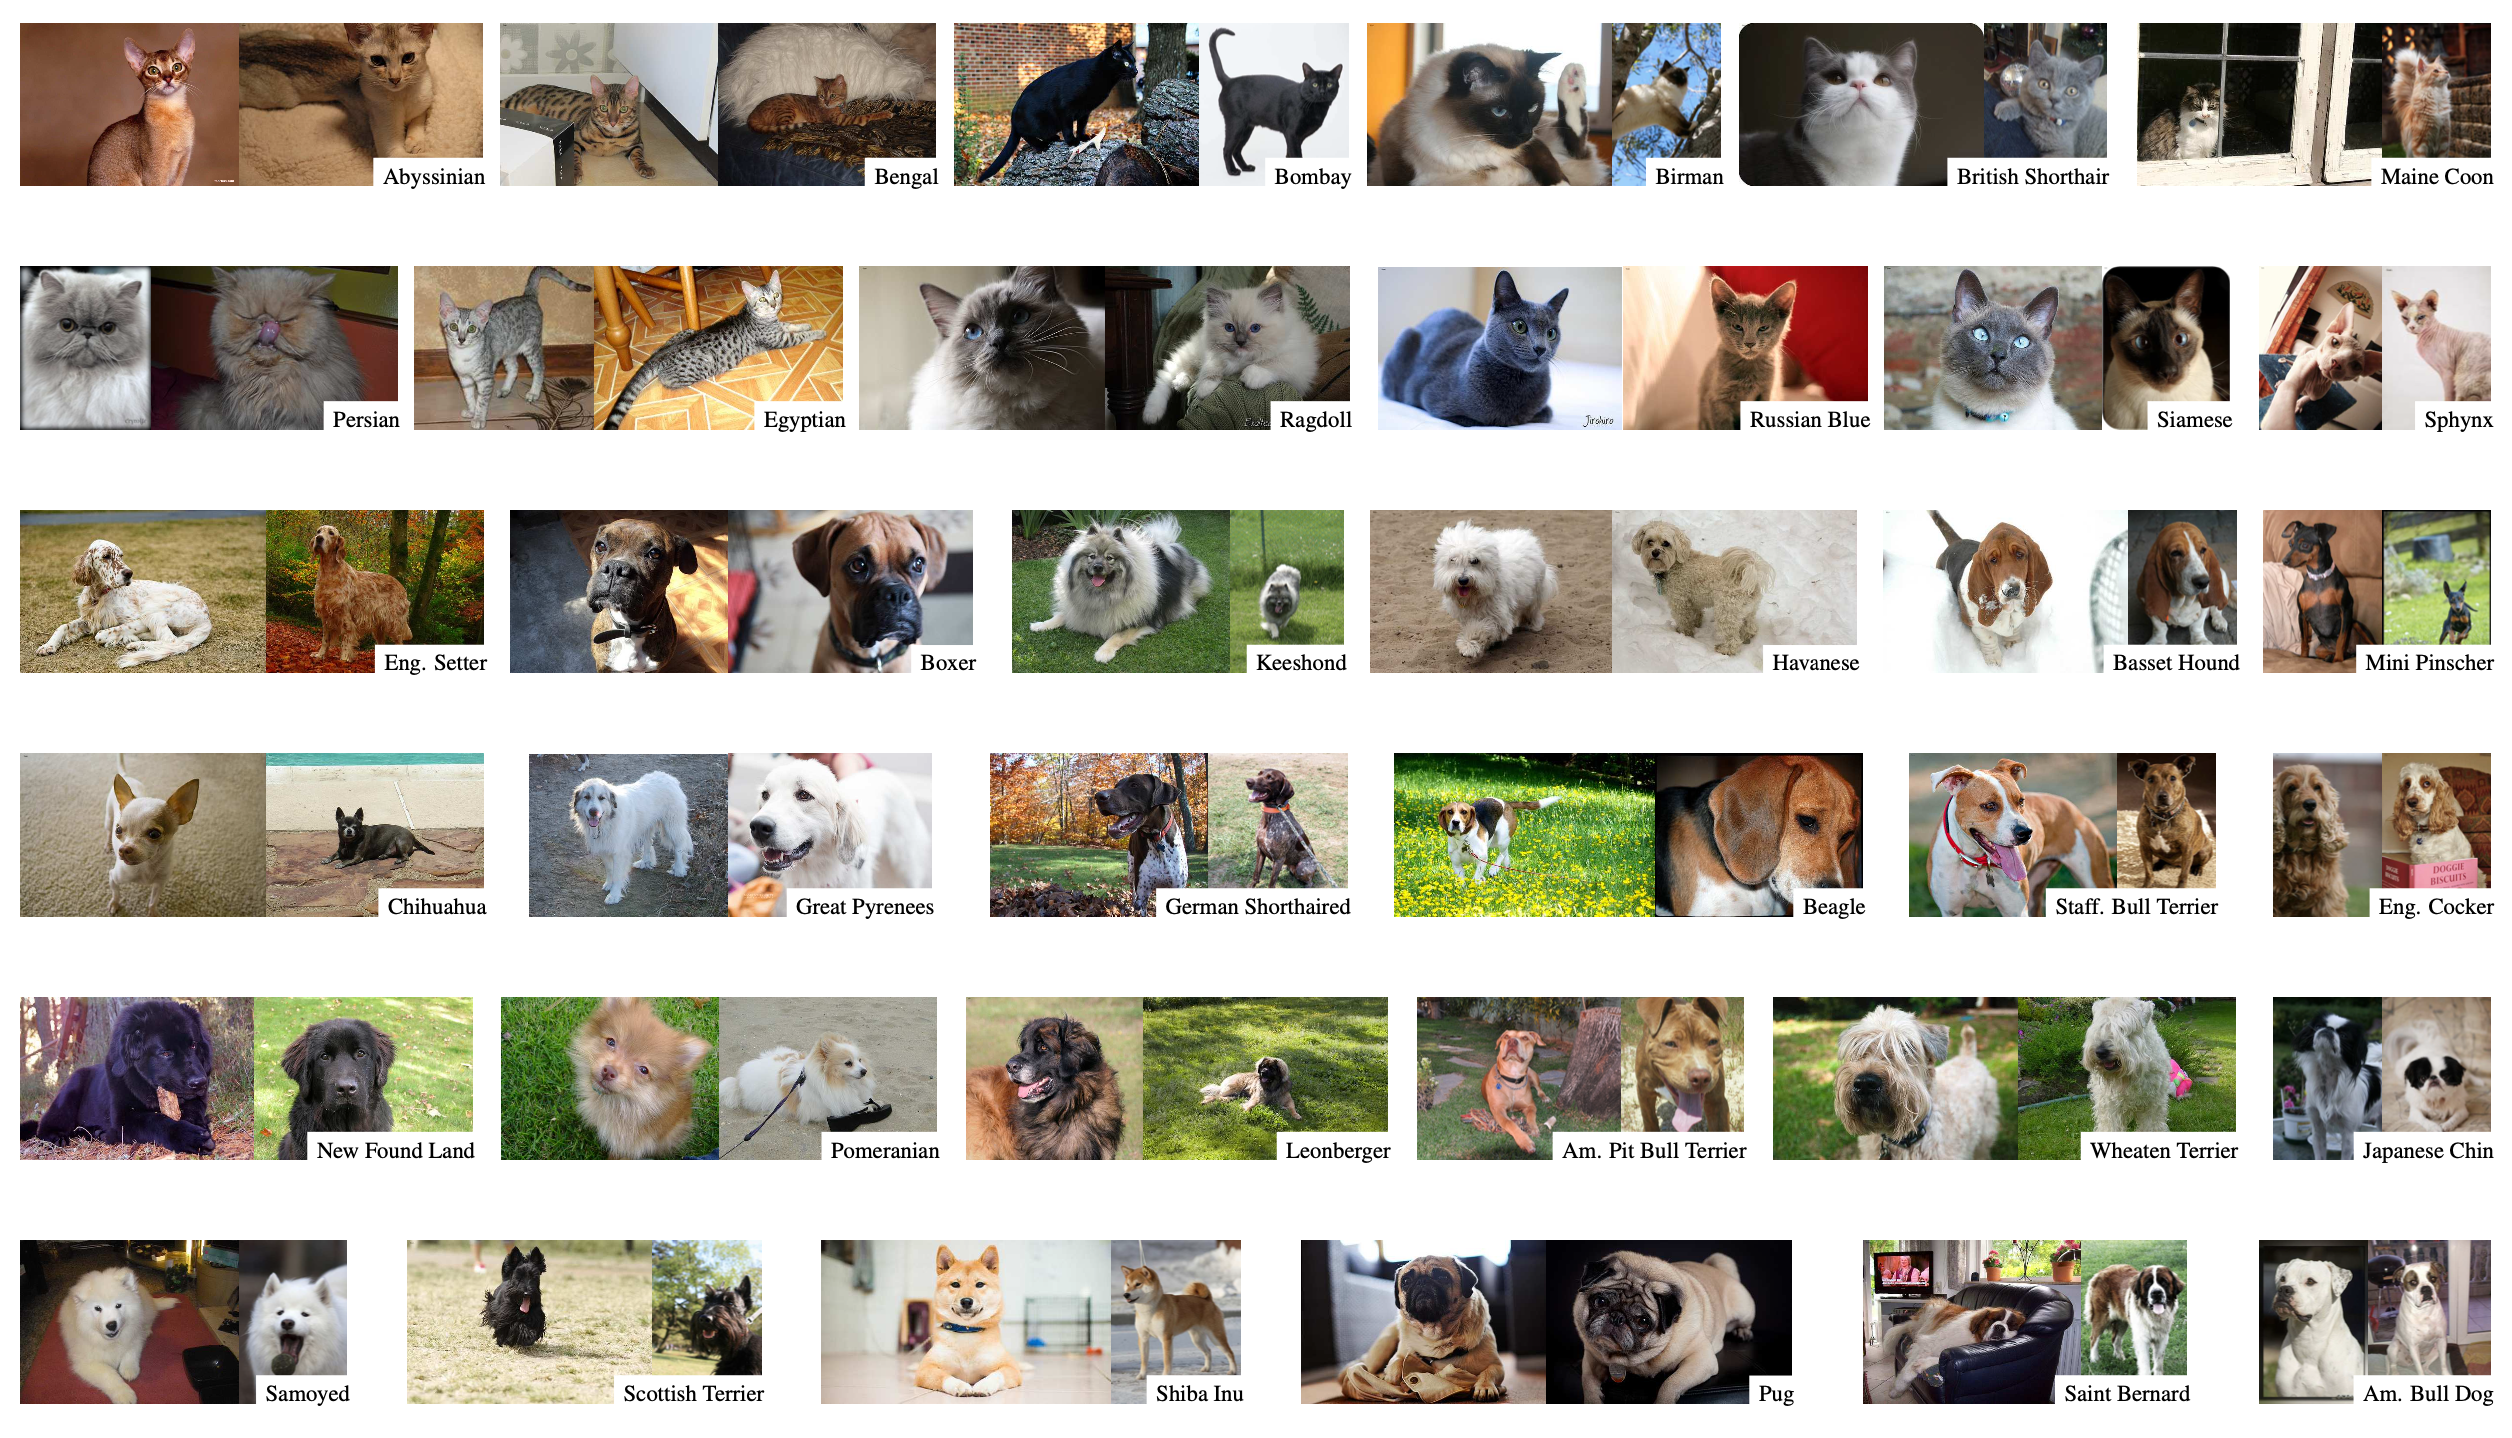
\includegraphics[width=1\textwidth]{Pictures/oxfordiiitPetC.png} 
    \caption{\textbf{Examples of each of the 37 Oxford-IIIT Pet classes} \cite{Parkhi2012CatsAD}. Note the significant variability found in the images, from changes in lighting and size to layout and scenery. This fact and the fact that it is a fine-grained dataset make it ideal for testing whether subject-driven augmentation is a competitive strategy.}
    \label{fig:oxfordiiitPetC}
\end{figure}

\begin{figure}
    \centering
    \includegraphics[width=1\textwidth]{Pictures/oxfordiiitPetS.png} 
    \caption{\textbf{Oxford-IIIT Pet annotations for segmentation}. Green is for the background region, yellow is for the ambiguous region, and purple is for the subject. }
    \label{fig:oxfordiiitPetS}
\end{figure}

We have chosen this dataset as the primary dataset for our analysis because it is fine-grained. This type of dataset contains many categories or classes with subtle distinctions between them. Unlike coarse-grained datasets with broader categories, fine-grained datasets focus on capturing fine details and subtle variations within a specific domain. Thus, given that the present work focuses on subject-driven augmentation techniques, such datasets allow us better discriminate the strengths and weaknesses of these techniques. In addition, the fact that this dataset contains both classification and segmentation annotations is also helpful.

On the other hand, the dataset used in experiment \textit{09-food-101} to show the versatility of the subject-driven augmentation technique is Food-101 \cite{bossard14}. This fine-grained dataset contains 101,000 images of 101 different food categories. We divide these images into 600 for training, 150 for validation and 250 for testing. It should be noted that both the training and validation images contain noise that the authors have not purposely cleaned to reflect that the real data is imperfect and contains large variability. Figure \ref{fig:food101} shows some images from this dataset showing the significant variability of the existing food types.

\begin{figure}
    \centering
    \includegraphics[width=1\textwidth]{Pictures/food101.png} 
    \caption{\textbf{Examples of 100 of the 101 Food-101 categories} \cite{bossard14}. Notice the significant variability of the existing food types and the fact that it is a fine-grained dataset.}
    \label{fig:food101}
\end{figure}

\subsection{Networks}
Concerning the deep network with which the experiments are carried out, the two proposed scenarios of classification and segmentation must be considered. For the first task, we take \textit{ResNet34}, a variant of the \textit{ResNet} architecture \cite{he2016deep} with 34 layers. This network is considered medium-sized, being smaller, for example, than \textit{ResNet50}. \textit{ResNet} stands for Residual Network, a reference to the residual connections that this architecture proposes to the problem of vanishing gradients. This problem occurs during the training of neural networks with methods based on gradient descent and backpropagation. The residual connections solution allows information to flow directly through the network layers, thus enabling the training of deeper networks. Figure \ref{fig:resnet34} shows the architecture of the \textit{ResNet34} network while comparing it with similar networks.

\begin{figure}
    \centering
    \includegraphics[width=0.5\textwidth]{Pictures/resnet34.png} 
    \caption{\textbf{Example network architectures for ImageNet and ResNet34} \cite{he2016deep}. The left column shows a \textit{VGG19} network as an example. The central one is a 34-layer network, which is modified on the right to form \textit{ResNet34} by adding the residual connections. The dotted line indicates an increase in dimension.}
    \label{fig:resnet34}
\end{figure}

Returning to the main problem of this work, we employ \textit{Resnet34} pre-trained on \textit{ImageNet-1k} and apply feature extraction with a fully connected classifier suitable for the 37 Oxford-IIIT Pet classes. The approach works because, even though the network is pre-trained, feature extraction allows us to exploit the meaningful features of the training images optimally. In this way, we can determine which data augmentation technique is the one that succeeds in making the extracted features as informative about the task as possible.

Finally, in the network training, Cross-Entropy is used as a loss function and stochastic gradient descent - SGD as an optimiser. Additionally, an early stopping with a patience of 5, a learning rate of $10^{-3}$ and a batch size of 16 are used.

On the other hand, for the segmentation task, we use the \textit{DeepLabV3} model \cite{chen2017rethinking} with \textit{ResNet101} as a backbone. The semantic segmentation architecture is based on the intensive use of \textit{atrous convolutions}. This type of convolution allows the expansion of the receptive field of a convolutional network without increasing the number of parameters. Figure \ref{fig:atrous} shows how this type of convolution works.

\begin{figure}
    \centering
    \includegraphics[width=0.6\textwidth]{Pictures/atrous.png} 
    \caption{\textbf{Atrous convolution with kernel size 3×3} \cite{chen2017rethinking}. The left image shows a standard convolution corresponding to a rate of 1. The other two images enlarge the rate and, therefore, the model's field of view. This allows objects of multiple scales to be considered in one image.}
    \label{fig:atrous}
\end{figure}

Returning to our segmentation task, we take a parallel approach to the classification task by performing feature extraction. In this case, the last layer of the \textit{DeepLabV3} model is modified so that the segmentation takes place in 3 values (subject, background and ambiguous region). Cross-Entropy is used as a loss function, and Adam as an optimiser. Additionally and analogously to the classification case, an early stopping with a patience of 5, a learning rate of $10^{-3}$ and a batch size of 16 are used.

\subsection{Subject-driven techniques and text-to-image model}

Stable Diffusion in its \textit{stable-diffusion-v1-5} version is used as a text-to-image model. The number of input images is 5, as can be seen from the results shown in \ref{sec: exp-01} and \ref{sec: exp-02}. The resolution of the generated synthetic images is 512x512. The rest of the model's parameters when generating the images are shown in table \ref{table:TableSDhyperparameters} and are derived from the analysis performed in \cite{stablediffusiondiffusers}.

\begin{table}[ht]
\centering
\begin{tabular}{|p{0.24\linewidth}|p{0.57\linewidth}|p{0.10\linewidth}|}
\hline
\rowcolor[HTML]{AEAAAA} 
\textbf{Hyperparameter} & \textbf{Description} & \textbf{Value} \\ \hline
\textit{num\_inference\_steps} & The bigger, the better the results are. However, also the longer the generation   takes & 50 \\ \hline
\textit{guidance\_scale} & It enhances the compliance with the conditional signal that directs the creation   (text). It compels the generation to align with the given prompt more closely, possibly sacrificing image quality or variety in the process. Also known as classifier-free guidance & 7.5 \\ \hline
\end{tabular}
\caption{\textbf{Stable Diffusion hyperparameters}}
\label{table:TableSDhyperparameters}
\end{table}

Table \ref{table:TableDreamboothhyperparameters} lists the hyperparameters with which Dreambooth is run. The choice of these is derived from the analysis of the Hugging Face blog \cite{dreamboothdiffusers}.

\begin{table}[ht]
\centering
\begin{tabular}{|l|p{0.48\linewidth}|l|}
\hline
\rowcolor[HTML]{AEAAAA} 
\textbf{Hyperparameter} & \textbf{Description} & \textbf{Value} \\ \hline
\textit{instance\_prompt} & Identifier specifying the instance & \textless{}funny-ret\textgreater{} \\ \hline
\textit{resolution} & Resolution for input images. All of them will be resized to that value & 512 \\ \hline
\textit{train\_batch\_size} & Batch   size for the training data loader & 1 \\ \hline
\textit{gradient\_accumulation\_steps} & Number   of updates steps to accumulate before performing a backward or update pass & 1 \\ \hline
\textit{learning\_rate} & Initial learning rate & $5\cdot10^{-6}$ \\ \hline
\textit{lr\_scheduler} & Scheduler type to use & constant \\ \hline
\textit{lr\_warmup\_steps} & Number of steps for the warmup in the \textit{lr\_scheduler} & 0 \\ \hline
\textit{max\_train\_steps} & Total number of training steps to perform & 400 \\ \hline
\end{tabular}
\caption{\textbf{Dreambooth hyperparameters}}
\label{table:TableDreamboothhyperparameters}
\end{table}

Table \ref{table:TableTextinversionhyperparameters} contains the hyperparameters with which Textual inversion is executed. Note that \textit{placeholder\_token} refers to the token used as a placeholder for the concept, \textit{initializer\_token} to the token used as the initialiser word and \textit{learnable\_property} as a choice between object or style.

\begin{table}[ht]
\centering
\begin{tabular}{|l|l|}
\hline
\rowcolor[HTML]{AEAAAA} 
\textbf{Hyperparameter} & \textbf{Value} \\ \hline
\textit{learnable\_property} & object \\ \hline
\textit{placeholder\_token} & \textless{}funny-ret\textgreater{} \\ \hline
\textit{initializer\_token} & animal \\ \hline
\textit{resolution} & 512 \\ \hline
\textit{train\_batch\_size} & 1 \\ \hline
\textit{gradient\_accumulation\_steps} & 4 \\ \hline
\textit{learning\_rate} & 5·10-4 \\ \hline
\textit{lr\_scheduler} & constant \\ \hline
\textit{lr\_warmup\_steps} & 0 \\ \hline
\end{tabular}
\caption{\textbf{Textual inversion hyperparameters}}
\label{table:TableTextinversionhyperparameters}
\end{table}

Finally, it is important to note that sometimes images generated by the text-to-image model are black and contain no information. This is because the Stable Diffusion model includes an NSFW content filter that is very easily activated. Therefore, the implementation made in this work does not consider these images. They are removed, and others are generated in their place.

\subsection{Hardware and environment}

The execution environment uses the resources provided by the Technical University of Denmark - DTU through the high-performance cluster - HPC belonging to the DTU Computing Center - DCC. The use of these advanced computing resources is because the tasks proposed in this work require significant amounts of processing power and memory. For more details about the hardware used, please refer to Appendix \ref{APHardware}. 

On the other hand, as for the software used. The programming language chosen to create the code is Python, in its version 3.8.13. The deep learning library, Pytorch in its version 2.0.1. Furthermore, as for the library containing the state-of-the-art pre-trained diffusion models as well as the subject-driven and conditional control techniques, Hugging Face diffusers has been used in version 0.16.1. For further details and a detailed list of all the libraries and software tools used, please visit Appendix \ref{APSoftware}.

\section{Results} \label{sec: results} 

This section shows the results obtained throughout the experiments defined in X. In addition, we accompany these results with relevant analyses and comments to allow the results to be interpreted in the context of the research question to be addressed in this paper in section \ref{sec:discussion}.

\subsection{Experiment 01-number-of-images} \label{sec: exp-01}

Experiment 1 studies the effect of the number of images used as input in Dreambooth and Textual inversion. Image \ref{fig:exp1} summarises the results of the experiment. It distinguishes the images used as input on the left and the resulting images on the right. Within the synthetic images, we provide the results of two prompts and 4 different values of images used as input for both Dreambooth and Textual inversion.   

\begin{figure}
    \centering
    \includegraphics[width=0.90\textwidth]{Pictures/exp1.png} 
    \caption{\textbf{Experiment 01-number-of-images}. The input images are shown on the left and the resulting images on the right. Synthetic images with two prompts and four input images variations for Dreambooth and Textual inversion are included.}
    \label{fig:exp1}
\end{figure}

Analysing these results is complex as it is an evaluation that does not rely on any easily measurable metric. However, the results suggest \textbf{better quality synthetic images are obtained using 5 real images} as input. To reach this conclusion, we looked at the generalisation ability of the subject in different contexts or positions. Thus, in the case of Textual inversion, it is clear that only in the case of 5 images the main characteristics of the creature are maintained. On the other hand, in the case of Dreambooth, we observe how the generalisation of the entity starts to be correct from the two input images. At this point, Dreambooth obtains more faithful results than Textual inversion.

In any case, we confirm that using a single image to execute these subject-driven techniques is unfeasible. This fact has important implications for our work. When using more than one image in a data augmentation use case with a real dataset, they are taken from the same class. Nevertheless, it is not assured that they are the same subject. In fact, in most cases, this will not be the case. This use case is not the primary use case of either Dreambooth or Textual inversion, and, therefore, we must ensure that, even with images of different subjects of the same class, these approximations work. In this line, special attention should be paid to experiment number 2, \textit{02-different-subjects}.

\subsection{Experiment 02-different-subjects} \label{sec: exp-02}

Experiment 2 studies how subject-driven techniques behave when the subjects of the input images are different. For this purpose, the dogs' domain is taken, and incrementally, Dreambooth and Textual inversion are used with increasingly different dogs. Image \ref{fig:exp2} summarises the results of the experiment. It distinguishes the images used as input at the top and the synthetic images for each technique at the bottom. In addition, for each technique, the synthetic images are divided into 4 subsets, each corresponding to a different subset of input images. The aim is to observe the differences in the images generated by the personalised text-to-image model with increasingly less similar inputs. Thus, the subsets of images used as input are:

\begin{itemize}
    \item \textbf{subset 1}: \textit{golden\_1, golden\_2, golden\_3.}
    \item \textbf{subset 2}: \textit{golden\_1, golden\_2, golden\_3, german\_1, german\_2.}
    \item \textbf{subset 3}: \textit{golden\_1, golden\_2, golden\_3, german\_1, german\_2, siberian\_1, siberian\_2.}
    \item \textbf{subset 4}: \textit{bulldog\_1, corgi\_1, german\_1, golden\_1, siberian\_1.}
\end{itemize}

\begin{figure}
    \centering
    \includegraphics[width=0.90\textwidth]{Pictures/exp2.png} 
    \caption{\textbf{Experiment 02-different-subjects}. The images used as input are at the top. The synthetic images for each technique are at the bottom. The experiment shows the differences in the images generated by the personalised text-to-image model with increasingly less similar inputs.}
    \label{fig:exp2}
\end{figure}

Analogous to the \textit{01-number-of-images} experiment, evaluating the images without an objective metric is problematic. However, the results obtained leave no doubt as to their quality. In all cases, subjects with dog-like characteristics are distinguishable in the synthetic images. It is especially noteworthy that, even with such different breeds as in \textit{subset\_4}, the images clearly show a being with dog characteristics. Although these images are readily identifiable as fake by the human eye, they contain very relevant information about what a dog is. Thus, with an appropriate architecture, they could be used to train a computer vision model. On the other hand, we would like to emphasise the magnificent results obtained with \textit{subset\_1}. With different subjects of the same breed (a fine-grained dataset if we make a parallelism with a computer vision task), Dreambooth and Textual inversion generate images that start to be difficult to distinguish from authentic images.

In summary, the \textit{02-different-subjects} experiment leaves no doubt that it is possible to use subject-driven techniques with different subjects of the same class. Therefore, these results support the idea that subject-driven augmentation techniques are an approach that should be considered in the training of complex computer vision tasks. Thus, we defined experiment \textit{03-training-percentage} to test subject-driven augmentation techniques on a real task.

\subsection{Experiment 03-training-percentage} \label{sec: exp-03}

Experiment 3 evaluates the entire subject-driven augmentation pipeline and compares it to other data augmentation techniques in a real task. This includes comparisons with the baseline, classical techniques and automated policies (AutoAugment and RandAugment). For subject-driven techniques, it includes Dreambooth, Textual inversion and Stable Diffusion prompt. In addition, the experiment examines the impact of varying the size of the real dataset. For this purpose, the percentage of data indicates how many images have been used. We consider 100\% the use of the complete Oxford-IIIT Pet training set. On the other hand, the number of synthetic images is kept fixed at 50.

Unlike the \textit{01-number-of-images} and \textit{02-different-subjects} experiments, we have a more rigorous evaluation method in this case. We use the accuracy of the trained model in the classification task and establish a baseline that does not employ any data augmentation technique. Figure X shows a plot of the results. 

\begin{figure}
    \centering
    \includegraphics[width=1\textwidth]{Pictures/experiment_003.pdf}
    \caption{\textbf{Experiment 03-training-percentage}. The experiment looks at how varying the size of the real dataset affects classic and subject-driven techniques. The percentage of data used is indicated on a logarithmic scale on the x-axis. We find that subject-driven augmentation techniques are a promising approach for small dataset sizes.}
    \label{fig:exp3}
\end{figure}

The data indicate that subject-driven augmentation techniques significantly improve model performance when the percentage of real data is 10\% or less. In this case, we observe significant increases in accuracy. For example, with 5\% real data, Textual inversion achieves a performance increase of 19.11\%. On the other hand, as we increase the number of real images to 10\%, the improvement achieved by Textual inversion is 3.37\%. From this point on, Textual inversion, despite being the most promising subject-driven approach, does not bring any new accuracy improvements that can be considered relevant. On the other hand, Dreambooth is the worst performer among the subject-driven techniques. This approach brings improvements of 16.06\% and 0.5\% when using 5\% and 10\% of the real data, respectively. Stable Diffusion prompt shows similar results to Textual inversion.

If we now look at the classical techniques (Custom data augmentation, AutoAugment and RandAugment), we can see how they worsen the accuracy when the dataset size is small. It is not until 50\% of the training set is present that they achieve performances that improve the baseline. Among them, RandAugment is the best performer, with accuracy increases of only 1.12\% when 100\% of the training set is used. In this case, all classical techniques can improve the result.

In summary, the data clearly show that subject-driven augmentation techniques are a promising approach when the dataset size is small. In this case, the training set contains 100 images per class when complete. Our results show that, for cases where data is scarce or very costly to obtain, one can take advantage of the capabilities and world knowledge of text-to-image models to increase the accuracy of classification models for computer vision tasks by more than 19\%. These findings are especially relevant since classical techniques fail miserably on small datasets.

\subsection{Experiment 04-generation-percentage} \label{sec: exp-04}

Experiment number 4 takes experiment \textit{03-training-percentage} and varies the percentage of images generated while leaving the size of the actual training set fixed. We consider two different scenarios. In the first one, we take 100\% of the Oxford-IIIT Pet training set and in the second one, only 5\%. Figure \ref{fig:exp4} shows a plot of the results. 

\begin{figure}
    \centering
    \includegraphics[width=0.93\textwidth]{Pictures/experiment_004.pdf}
    \caption{\textbf{Experiment 04-generation-percentage}. The experiment involves manipulating the proportion of generated data (measured on a logarithmic scale). Our findings indicate that in large datasets, the techniques do not yield a substantial improvement in system performance. However, in smaller ones, they do demonstrate an increase.}
    \label{fig:exp4}
\end{figure}

The data obtained show that when 100\% of the real training data is used (i.e. sufficient training data is available), it does not make sense to use subject-driven augmentation techniques. These approaches are not able to improve the baseline performance in a significant way. Moreover, the 3 techniques considered show a clear tendency to worsen their results as the number of synthetic images increases. 

On the other hand, using the subject-driven techniques makes much sense when using 5\% of the real training data (i.e., very little training data). By adding only a few images, the accuracy increases substantially. Adding only 100\% new synthetic images (which would imply doubling the number of images from 5 to 10), up to 18.93\% is achieved with Stable Diffusion prompt and 11\% with Textual inversion. In this scenario, increasing the number of synthetic images can improve the results, but only to a certain extent. By adding 1000\% synthetic images, Textual inversion offers a performance improvement of 19.11\%.

In summary, when there are enough training images, subject-driven augmentation techniques are not able to increase the performance of the system significantly, no matter how many synthetic images are added. In contrast, when the dataset is small, these approaches substantially improve the results.

\subsection{Experiment 05-all-generated} \label{sec: exp-05}

\subsection{Experiment 06-controlnet} \label{sec: exp-06}


\subsection{Experiment 07-combinations} \label{sec: exp-07}


\begin{table}[ht]
\centering
\begin{tabular}{|p{0.45\linewidth}|l|l|l|}
\hline
\cellcolor[HTML]{BFBFBF}\textbf{Description} & \cellcolor[HTML]{BFBFBF}\textbf{Real   data} & \cellcolor[HTML]{BFBFBF}\textbf{Synthetic   data} & \cellcolor[HTML]{BFBFBF}\textbf{Variation} \\ \hline
Textual inversion + RandAugment & 100\% & 100\% & -1,43\% \\ \hline
Textual inversion + RandAugment & 100\% & 50\% & -1,24\% \\ \hline
Textual inversion + RandAugment & 100\% & 10\% & 0,61\% \\ \hline
Textual inversion + RandAugment & 100\% & 5\% & -1,48\% \\ \hline
Dreambooth + RandAugment & 100\% & 5\% & 0,12\% \\ \hline
Stable Diffusion prompt + RandAugment & 100\% & 10\% & -0,18\% \\ \hline
Stable Diffusion prompt + RandAugment & 100\% & 5\% & -0,25\% \\ \hline
ControlNet + RandAugment & 100\% & 100\% & -0,25\% \\ \hline
ControlNet + RandAugment & 100\% & 5\% & -1,53\% \\ \hline
Textual inversion + RandAugment & 5\% & 1000\% & -1,83\% \\ \hline
Stable Diffusion prompt + RandAugment & 5\% & 200\% & 1,83\% \\ \hline
ControlNet + RandAugment & 5\% & 2000\% & -7,23\% \\ \hline
\end{tabular}
\caption{\textbf{Exp 07}}
\label{table:TableExp07}
\end{table}

\subsection{Experiment 08-segmentation} \label{sec: exp-08}

\subsection{Experiment 09-food-101} \label{sec: exp-09}



LOS APENDICES CON LAS IMAGEN GENERADAS. ESO NO LO HE PUESTO Y TENDRIA QUE HABER EMPEZADO A DECIRLO EN EL 03.